\documentclass{beamer}
\usepackage[utf8]{inputenc}
\usepackage[T1]{fontenc}
\usepackage{graphicx, caption,wrapfig}
\usepackage{siunitx,physics}

% \usepackage{algorithmicx}
% \usepackage{algorithm}
% \usepackage[noend]{algpseudocode}

\title{A Multigrid Poisson Solver for PINC}
\date{\today}
\author[Author]{Gullik V. Killie \hspace*{3.6cm}Wojciech J. Miloch}

\usetheme{uio}

\usepackage[style=authoryear,
            bibstyle=authoryear,
            backend=biber,
            % refsection=chapter,
            maxbibnames=99,
            maxnames=2,
            firstinits=true,
            uniquename=init,
            natbib=true,
            dashed=false]{biblatex}


\addbibresource{bib.bib}

%%%%%%%%%%%%%%%%%%%%%%%%%%%%%%%%%%%%%%%%%%%%%%%%%%%%%%%%%%%%%%%%%%%
%Tikz settings
% =================================================
% % Set up a few colours
% \colorlet{lcfree}{Green3}
% \colorlet{lcnorm}{Blue3}
% \colorlet{lccong}{Red3}
% -------------------------------------------------
% Set up a new layer for the debugging marks, and make sure it is on
% top
\pgfdeclarelayer{marx}
% \pgfsetlayers{main,marx}
% A macro for marking coordinates (specific to the coordinate naming
% scheme used here). Swap the following 2 definitions to deactivate
% marks.
\providecommand{\cmark}[2][]{%
  \begin{pgfonlayer}{marx}
    \node [nmark] at (c#2#1) {#2};
  \end{pgfonlayer}{marx}
  }
\providecommand{\cmark}[2][]{\relax}


% TikZ environment initialisation
\usetikzlibrary{calc,fadings,decorations.pathreplacing,decorations.markings}
\usetikzlibrary{shapes,arrows,chains}
% \usetikzlibrary{fadings,shapes.arrows,shadows}
% \usetikzlibrary{arrows,external,pgfplots.groupplots,positioning}
% \usetikzlibrary{intersections}
\usetikzlibrary{decorations.pathmorphing,patterns}
% Setting colours used
\definecolor{royalBlue}{RGB}{65,105,225}
\definecolor{cadred}{RGB}{227,0,34}
\definecolor{slateGray}{RGB}{119,136,153}

% TikZ style def.
\tikzset{
    %Define style for boxes
    >=stealth,
    punkt/.style={
           rectangle,
           rounded corners,
           draw=white, very thick,
           text width=10em,
           minimum height=2em,
           text centered},
    % Define arrow style
    pil/.style={
           ->,
           >=stealth,
           thick,
           shorten <=2pt,
           shorten >=2pt},
    % Define a box style for grid
    box/.style={
          rectangle,
          draw=black,
          thin,
          minimum size=0.1cm},
    circ node/.style={
          circle,
          draw,
          inner sep=4pt},
    % style to apply some styles to each segment of a path
    spring1/.style={
      decoration={
        aspect=1,
        segment length=1.448cm,
        % segment length=0.38cm,
        amplitude=0.3cm,
        coil,
      },
    },
    spring2/.style={
      decoration={
        aspect=0.399,
        segment length=0.601cm,
        amplitude=0.75cm,
        coil,
      },
    },
    % style to add an arrow in the middle of a path
    mid arrow/.style={postaction={decorate,decoration={
          markings,
          mark=at position .3 with {\arrow[#1]{stealth}}
    }}},
    extended line/.style={shorten >=-#1,shorten <=-#1},
}

% \AtBeginSection[]
% {
%   \begin{frame}<beamer>
%     \frametitle{Outline for section \thesection}
%     \tableofcontents[currentsection]
%   \end{frame}
% }
\begin{document}
%----------------- Build title page and tableofcontents ---
\begin{frame}
\titlepage
\end{frame}
%
\begin{frame}{Overview}
\tableofcontents
\end{frame}
% ---------------- Start presentation slides below --------
\begin{frame}
	\frametitle{Aim of the Thesis}
	\begin{itemize}
		\item Develop a new Parallel Multigrid solver for the new Particle-in-Cell model PINC
	\end{itemize}
\end{frame}
\section{Background} % (fold)
\label{sec:Background}
\begin{frame}
	\frametitle{Plasma}
	\framesubtitle{Why Plasma}
	\begin{columns}
	\column{0.5\linewidth}
		\begin{itemize}
			\item Appears in various important areas that affect us
			\item The Sun, Upper parts of the Earth's Atmosphere
			\item Important industrial applications
			\item Plasma cutters, light tubes/bulbs, fusion
		\end{itemize}
	\column{0.5\linewidth}
		\begin{figure}
			\centering
			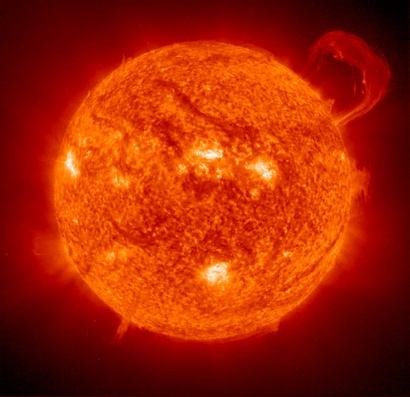
\includegraphics[width = \textwidth]{figures/sun}
			\caption{Picture of the sun, taken with SOHO's Extreme ultraviolet Imaging Telescope \citep{_sun_????}}
		\end{figure}
	\end{columns}
\end{frame}
%
\begin{frame}
	\frametitle{Plasma}
	\framesubtitle{What is Plasma}
	\indent \textit{\large"A plasma is a quasineutral gas of charged and neutral particles which exhibits
	collective behaviour."}
	\begin{flushright}
	    \textbf{Francis F. Chen} \citep{chen_introduction_1984}\\[1.0cm]
	\end{flushright}
	\begin{itemize}
		\item Neutral and charged particles
		\item Electromagnetic forces due to the charge
	\end{itemize}
\end{frame}

\begin{frame}
	\frametitle{Plasma}
	\framesubtitle{Governing Equations}
	\only<1>{\framesubtitle{Frame subtitle 4}
	\begin{block}{Equations of motion}
	\begin{subequations}
		\begin{align*}
		m\dv{\vb v(t)}{t} &= q[\vb E(\vb r(t),t) + \vb v(t) \times \vb B(\vb r(t),t)]\\
		\dv{\vb r(t)}{t} &= \vb v(t)
		\end{align*}
	\end{subequations}
	\end{block}
	\begin{block}{Maxwell's equations}
	\begin{subequations}
	\begin{align*}
	\nabla \cdot \vb E &= \frac{\rho}{\varepsilon_0}  &  \nabla \cdot \vb B &= 0 \\
	\nabla \times \vb E &= -\frac{\partial \vb B}{\partial t} &  \nabla \times \vb B &= \mu_0 \vb J + \mu_0\varepsilon_0 \frac{\partial \vb E}{\partial t}
	\end{align*}
	\end{subequations}
	\end{block}
	}
\end{frame}

% section introduction (end)
%
\section{Particle-in-Cell} % (fold)
\label{sec:sec2}
% \subsection{subsection1} % (fold)
\label{sub:ssec1}
\begin{frame}
	\frametitle{Particle-in-Cell}
	\framesubtitle{Overview}
		% \only<1-2>{\begin{itemize}
		% \item \only<1->{ item 1}
		\begin{itemize}
			\item Particle based - Computes the Equations of Motion for each particle
			\item Each particle is interacting with a field, instead of all the other particles
		\end{itemize}
	% \end{itemize}}
	\centering
\end{frame}
\begin{frame}
	\frametitle{Particle-in-Cell}
	\framesubtitle{Components}
	\begin{figure}
		\center
		\resizebox{11.cm}{3.cm}{
			
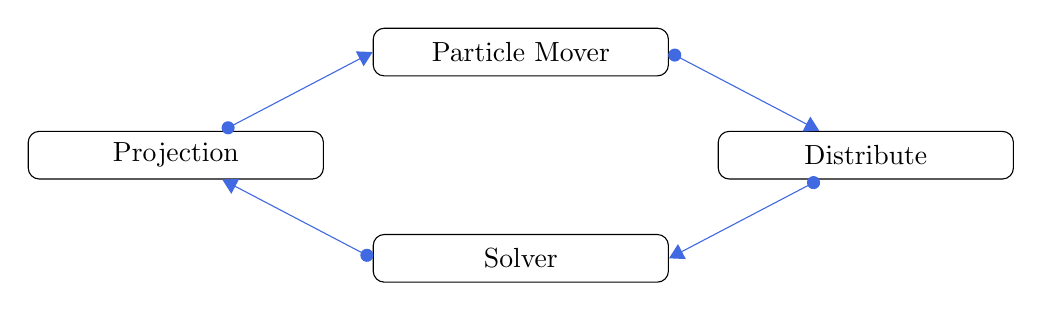
\begin{tikzpicture}[
    >=triangle 60,              % Nice arrows; your taste may be different
    start chain=going below,    % General flow is top-to-bottom
    node distance=10mm and 25mm, % Global setup of box spacing
    every join/.style={norm},   % Default linetype for connecting boxes
    scale=0.1]
% -------------------------------------------------
% A few box styles
% <on chain> *and* <on grid> reduce the need for manual relative
% positioning of nodes
\tikzset{
  base/.style={draw, on chain, on grid, align=center, minimum height=4ex},
  proc/.style={base, rectangle, text width=10em},
  test/.style={base, diamond, aspect=2, text width=5em},
  term/.style={proc, rounded corners},
  % coord node style is used for placing corners of connecting lines
  coord/.style={coordinate, on chain, on grid, node distance=6mm and 45mm},
  % nmark node style is used for coordinate debugging marks
  nmark/.style={draw, cyan, circle, font={\sffamily\bfseries}},
  % -------------------------------------------------
  % Connector line styles for different parts of the diagram
  norm/.style={->, draw, royalBlue},
  free/.style={->, draw, cadred},
  cong/.style={->, draw, slateGray},
  it/.style={font={\small\itshape}}
}
% -------------------------------------------------
% Start by placing the nodes
\node[term] (move) {Particle Mover};
\node[coord] (center) {};
\node[term]	(field) {Solver};
\node[term, right =of center] (density) {Distribute};
\node[term, left =of center] (force) {Projection};

%Lines
\draw [*->, royalBlue, yshift = -1em] (move.east) -- (density);  %MAke curved if time
\draw [*->, royalBlue] (density) -- (field.east);  %MAke curved if time
\draw [*->, royalBlue] (field.west) -- (force);  %MAke curved if time
\draw [*->, royalBlue] (force) -- (move.west);  %MAke curved if time

\end{tikzpicture}

		}
		\caption{Schematic overview of the electrostatic PIC cycle. The mover moves all the particles and updates their velocities.
		Next the particle charges are distributed to a charge density grid. The solver then
		obtains the electric field on the grid (and magnetic field in a full electromagnetic model when also the currents are weigthed to the grid). Lastly the field values are
		projected onto the particles.}
		\label{fig:schematic}
	\end{figure}
\end{frame}
\begin{frame}
	\frametitle{Particle-in-Cell}
	\framesubtitle{Components}
	\begin{itemize}
		\item Mover - Moves all the particles
		\item Distribute - Distributes the charges from the particles onto the grid
		\item Solver - Solves the equation on the grid -> obtains electric potential
		\item Projection - Field values projected onto the particles
	\end{itemize}
\end{frame}
%
\section{Multigrid} % (fold)
\label{sub:ssec2}%
\begin{frame}
	\frametitle{Multigrid}
	\begin{itemize}
		\item Solves the Poisson equation, \(\epsilon_0 \nabla \cdot \vec{E} = e(n_i-n_e)\).
		\item Charge distribution (\(\rho\)) \(\longrightarrow\) Potential (\(\Phi\))
		\item Solves the problem on different grid resolutions
	\end{itemize}
\end{frame}

\begin{frame}
	\frametitle{Multigrid}
	\framesubtitle{Schematic overview}
	\begin{figure}
		\center
		\resizebox{10.cm}{6.cm}{
			% %Figure
\begin{figure}
    \center
    \begin{tikzpicture}[%
        >=triangle 60,              % Nice arrows; your taste may be different
        start chain=going below,    % General flow is top-to-bottom
        node distance=6mm and 2mm, % Global setup of box spacing
        every join/.style={norm},   % Default linetype for connecting boxes
        scale = 1]
        % -------------------------------------------------
        % A few box styles
        % <on chain> *and* <on grid> reduce the need for manual relative
        % positioning of nodes
        \tikzset{
        base/.style={draw, on chain, on grid, align=center, minimum height=8ex, color = black},
        proc/.style={base, rectangle, text width=5em},
        % test/.style={base, diamond, aspect=2, text width=5em},
        term/.style={proc},
        % coord node style is used for placing corners of connecting lines
        coord/.style={coordinate, on chain, on grid, node distance=6mm and 9mm},
        point/.style={draw, circle, thick ,color = black},
        % nmark node style is used for coordinate debugging marks
        move/.style={draw, blue,rounded corners, fill=white, text = black, align = left},
        comp/.style={text = black}
        % -------------------------------------------------
        % Connector line styles for different parts of the diagram
        norm/.style={->, draw, lcnorm},
        free/.style={->, draw, lcfree},
        cong/.style={->, draw, lccong},
        it/.style={font={\small\itshape}}
        }
        % -------------------------------------------------
        % Start by placing the nodes
        \node[term] (U) {0};

        \node[coord, below =of U] (U1)      {};
        \node[coord, below =of U1] (U2) {};
        \node[coord, below =of U2] (U3) {};
        \node[coord, below =of U3] (U4) {};
        \node[coord, below =of U4] (U5) {};
        \node[coord, right =of U5] (U6) {};

        \node[term, right =of U6] (V) {1};

        \node[coord, below =of V] (V1) {};
        \node[coord, below =of V1] (V2) {};
        \node[coord, below =of V2] (V3) {};
        \node[coord, below =of V3] (V4) {};
        \node[coord, below =of V4] (V5) {};
        \node[coord, right =of V5] (V6) {};

        \node[term, right =of V6] (W) {2};

        \node[coord, above =of W] (Wup1) {};
        \node[coord, above =of Wup1] (Wup2) {};
        \node[coord, above =of Wup2] (Wup3) {};
        \node[coord, above =of Wup3] (Wup4) {};
        \node[coord, above =of Wup4] (Wup5) {};
        \node[coord, right =of Wup5] (Wup6) {};

        \node[term, right =of Wup6] (Vup) {1};

        \node[coord, above =of Vup] (Vup1) {};
        \node[coord, above =of Vup1] (Vup2) {};
        \node[coord, above =of Vup2] (Vup3) {};
        \node[coord, above =of Vup3] (Vup4) {};
        \node[coord, above =of Vup4] (Vup5) {};
        \node[coord, right =of Vup5] (Vup6) {};


        \node[term, right =of Vup6] (Uup) {0};

        %Top level Equations
        \node[point, left =of U]  { \(1\)};

        \node[point, right =of Uup]	{ \(5\)};

        %Center level
        \node[point, left =of V]   { \(2\)};

        \node[point, right =of Vup]   { \(4\)};

        %Bottom level
        \node[point, left =of W]	{ \(3\)};

        \draw[*->, lccong] (U) -- (V) node[move, midway] {Restrict};
        \draw[*->, lccong] (V) -- (W) node[move, midway] {Restrict};
        \draw[*->, lccong] (W) -- (Vup) node[move, midway] {Prolongate};
        \draw[*->, lccong] (Vup) -- (Uup) node[move, midway] {Prolongate};

        \draw[bend right = 50t,*->, thick]  (Uup) to node [auto, swap] {Repeat} (U);
    \end{tikzpicture}
    \caption{Schematic overview of the PIC method. In a three level MG implementation, there is 5 main steps in a cycle that needs to be considered.}
    \label{fig:MG_schematic}
\end{figure}

		}
		\caption{Schematic overview of the Multigrid cycle. In a three level MG V implementation,
			there is 5 main steps in a cycle that needs to be considered.}
	\end{figure}
\end{frame}

\begin{frame}
	\frametitle{Multigrid}
	\framesubtitle{Algorithm}
	\begin{figure}
	\center
	\resizebox{10.cm}{6.cm}{
	\tikzstyle{blank} = [circle,minimum size=10pt,inner sep=0pt]
\tikzstyle{texting} = [circle,minimum size=10pt,inner sep=0pt]



\begin{tikzpicture}[scale = 1.45, auto,swap]
    \node[blank] (start) at (0,5) {};
    \node[blank] (bot_start) at (2,0) {};
    \node[blank] (bot_end) at (8,0) {};
    \node[blank] (end) at (10,5) {};
    %Draw lines
    \draw[*->] (start) -- (bot_start);
    \draw[*->] (bot_start) -- (bot_end);
    \draw[*->] (bot_end) -- (end);
    %Put in Algorithm steps
    %Downwards
    \node[texting] (haloDown)       at (1.2,4.5) {HaloBnd($\phi$)};
    \node[texting] (smoothDown)     at (1.7,3.5) {Smooth($\phi, \rho$)};
    \node[texting] (haloDown2)      at (1.7,2.5) {Halo($\rho$)};
    \node[texting] (resDown)        at (2.7,1.5) {Residual($\text{res},\phi,\rho$)};
    \node[texting] (restrict)       at (2.9,0.5) {Restrict($\text{res},\rho$)};
    %Bottom
    \node[texting] (halo1)      at (2.5,-0.5) {Halo($\rho$)};
    \node[texting] (smooth1)    at (4.3,-0.5) {Smooth($\phi,\rho$)};
    \node[texting] (halobnd)    at (6.1,-0.5) {HaloBnd($\phi$)};
    \node[texting] (prol)       at (7.6,-0.5) {Prol($\rho$)};
    %Upwards
    \node[texting] (sub)        at (7.4,1.0) {Sub($\phi,\text{res}$)};
    \node[texting] (halobndUp)  at (7.8,2.0) {HaloBnd($\phi$)};
    \node[texting] (smoothUp)   at (8.2,3.0) {Smooth($\phi$)};
    \node[texting] (prolongate) at (8.2,4.0) {Prolongate($\text{res},\phi$)};
\end{tikzpicture}
 }
	\caption{The algorithmic steps in a 2-level Multigrid algorithm}
	\end{figure}
\end{frame}

\begin{frame}
	\frametitle{Multigrid}
	\framesubtitle{Components}
	\begin{itemize}
		\item HaloBnd - Fill Ghost cells according to boundary condition
		\item Smooth - Solve with Gauss-Seidel RB
		\item Halo - Compute Residual
		\item Restrict - Go to coarser grid
		\item Retrieve improvement to solution from coarser grid
		\item Smooth - Improve solution
	\end{itemize}
\end{frame}


\section{Results}
\subsection{Verification}

\begin{frame}
	\frametitle{Results}
	\framesubtitle{Overview}
		\begin{itemize}
			\item Verification Multigrid module
			\item Verification PINC
			\item Scaling
		\end{itemize}
\end{frame}

\begin{frame}
	\frametitle{Results}
	\framesubtitle{Verification Multigrid module}
	Tested on:
	\begin{itemize}
		\item Analytical solutions of sinusoidal and Heaviside charge distributions
		\item Random charge distributions
		\item \(2\) different algorithms (ND and 3D) was tested against each other
		\item Scaling of the error due to discretization
		\item Performed well on all the test
	\end{itemize}
\end{frame}
\begin{frame}
	\frametitle{Results}
	\framesubtitle{Heaviside}
		\begin{figure}
		\includegraphics[scale = 0.3]{figures/verification/rho}
		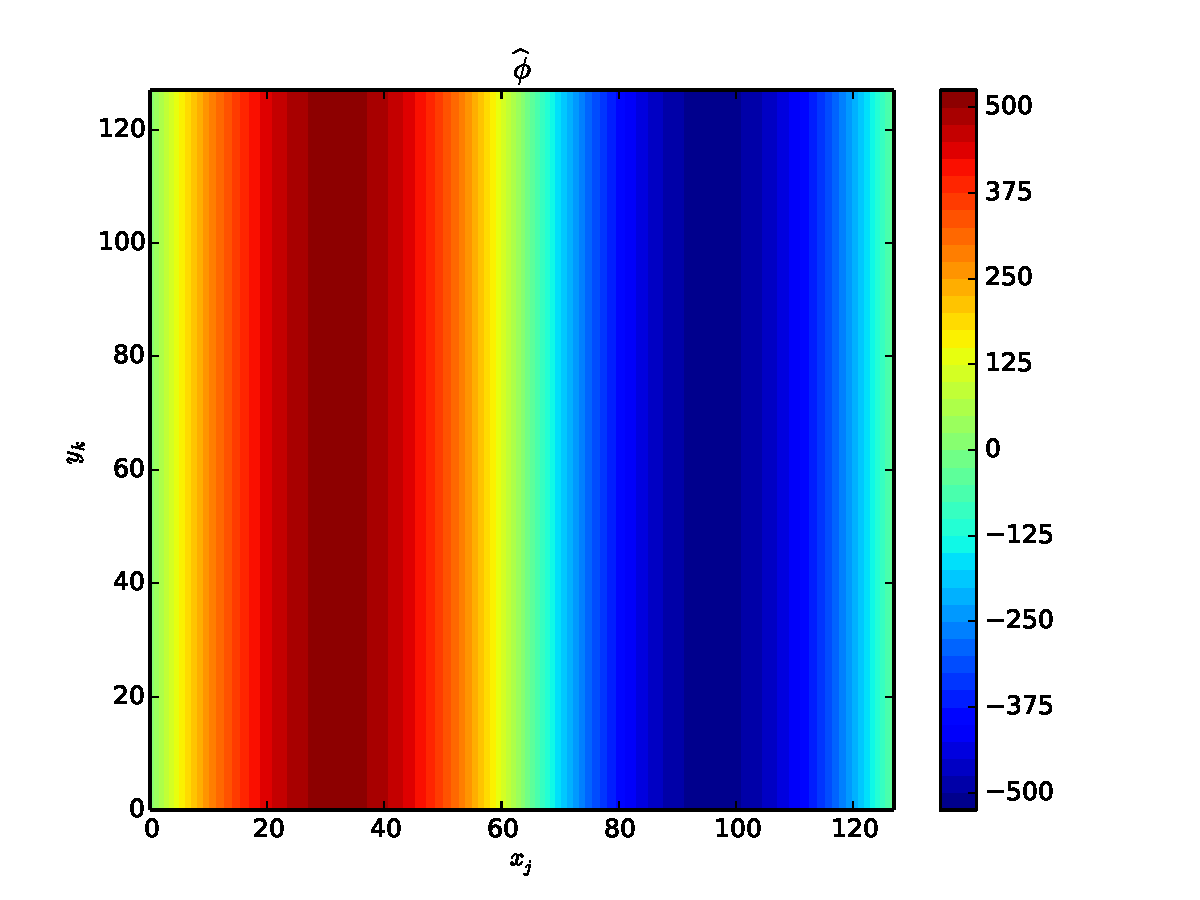
\includegraphics[scale = 0.3]{figures/verification/numerical}
		\caption{Slice of the charge distribution (left) and the numerical solution (right) for the resulting potential. The
		resulting potential has the expected \(2\)nd degree polynomial shape. The residual was on the order \(10^{-5}\).}
		\end{figure}
\end{frame}

\begin{frame}
	\frametitle{Results}
	\framesubtitle{Discretization Error}
	    \centering
	\begin{figure}
        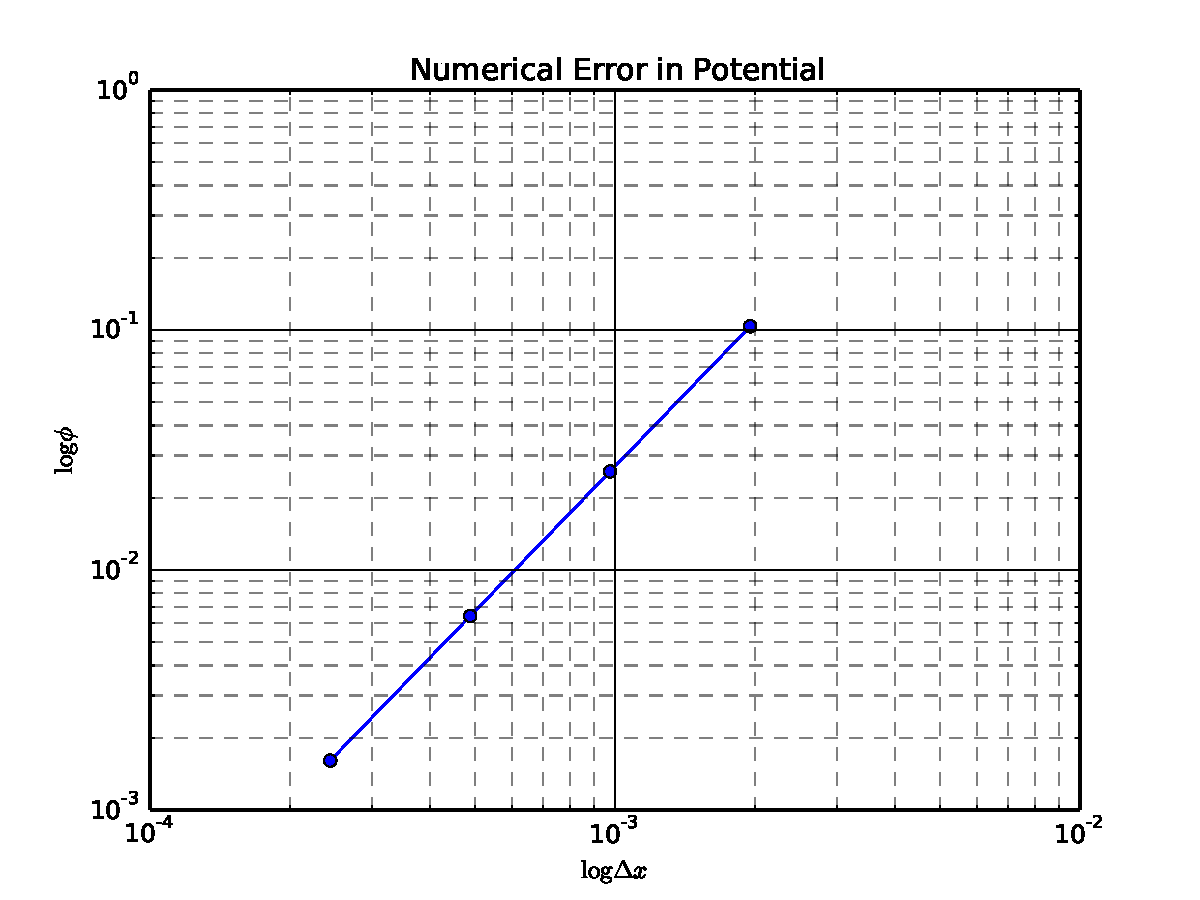
\includegraphics[width = 0.4\textwidth]{figures/verification/errorloglogPotential}
		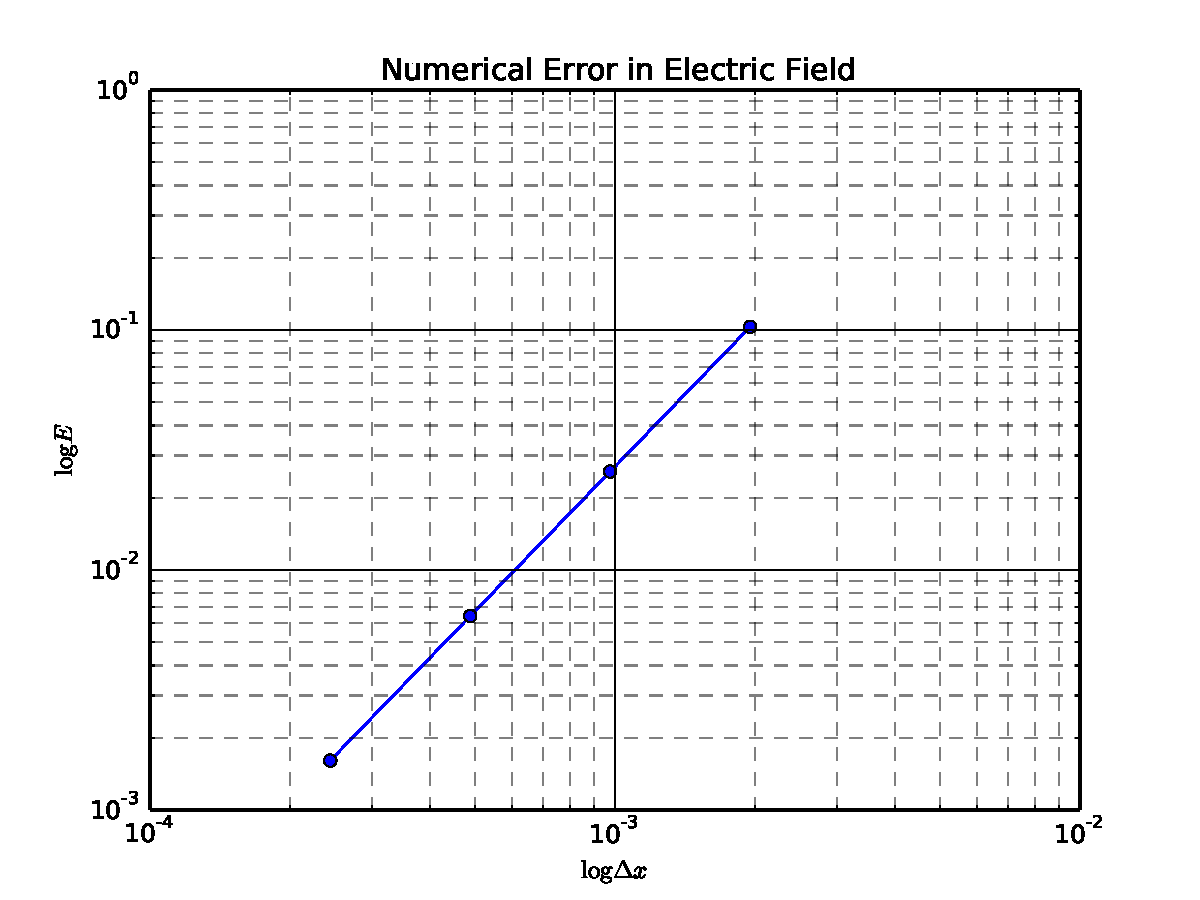
\includegraphics[width = 0.4\textwidth]{figures/verification/errorloglogE}
	    \caption{Logarithmic plot of the 2-norm of the error of the potential \(\phi\) (left) and the
	    x-component of the electric field. The solver was run on a scaled sinus-shaped charge distribution.
	    Both of the plots show a straight line of the error, on the logarithmic plots, with a slope
	    of \(2.00\). This corresponds to the error scaling with order \(-2\) as a function of the
		stepsize as expected. All the units are in PINC normalized units.}
	    \label{fig:errorScaling}
	\end{figure}
\end{frame}

\begin{frame}
	\frametitle{Results}
	\framesubtitle{PINC - Verification}
		\begin{itemize}
			\item PINC was tested by reproducing a Langmuir Plasma Oscillation
		\end{itemize}
		\begin{figure}
			\label{fig:oscillation}
			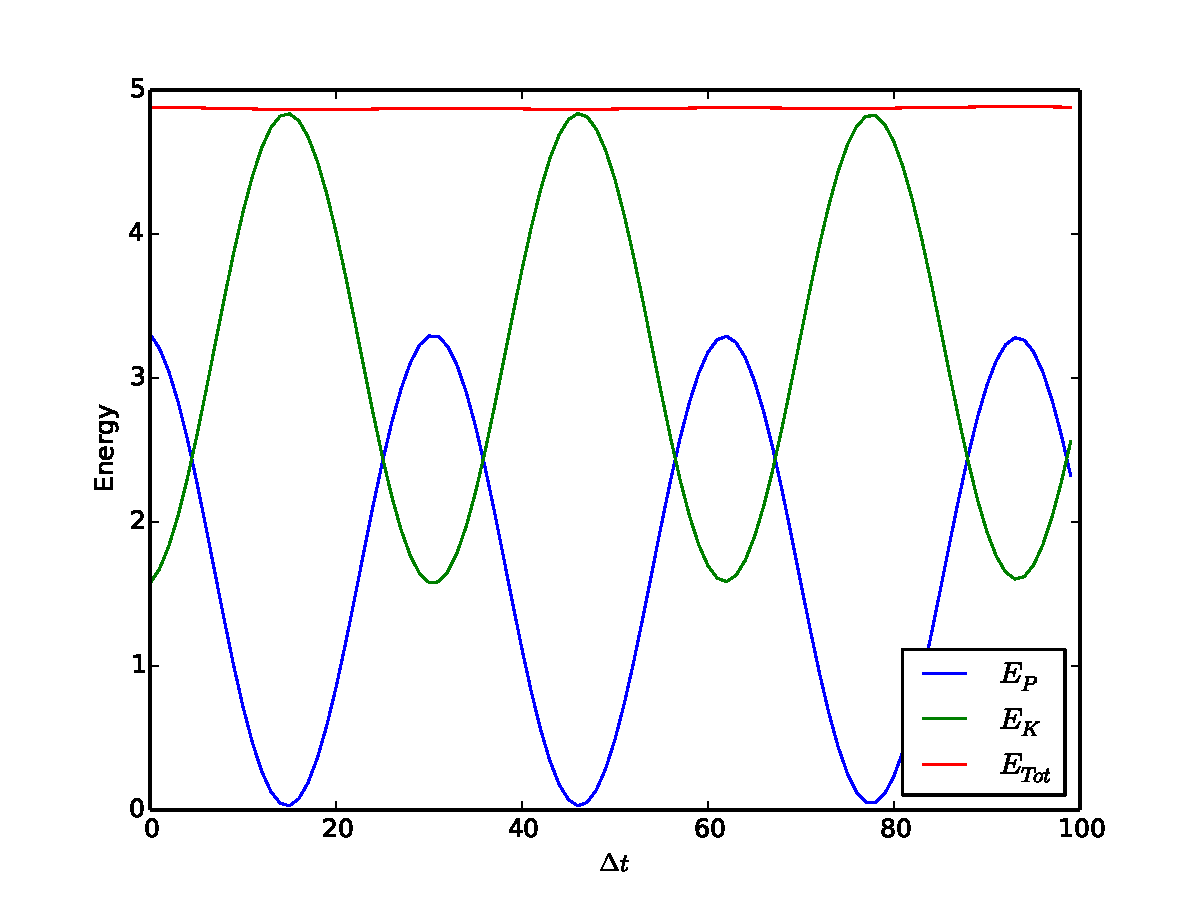
\includegraphics[width = 0.5\textwidth]{figures/verification/energyPlot}
			\caption{This shows the time-evolution of the energy in an perturbed plasma. The energies are
			in normalized units and \(\Delta x = 0.1 \lambda_{De}\). The total energy has a maximum variation of \(0.22\%\). In the timespan
			of \(10\omega_{pe}\) the plasma oscillates over \(1.6\) times.}
		\end{figure}
\end{frame}

\subsection{Parallel Scaling}
\begin{frame}
	\frametitle{Results}
	\framesubtitle{Parallel Scaling}
	Parallel Scaling of the Multigrid Solver
	\begin{itemize}
		\item Tested by increasing the problem (\# grid points), with a corresponding increase in processors
		\item Timing how long it took to solve the problem satisfactorily
		\item Scaling was tested on the Abel supercomputer at UiO
	\end{itemize}
\end{frame}

\begin{frame}
	\frametitle{Results}
	\framesubtitle{Parallel Scaling}
	\begin{figure}
		% \begin{subfigure{\textwith}
		\label{fig:scalingMG}
		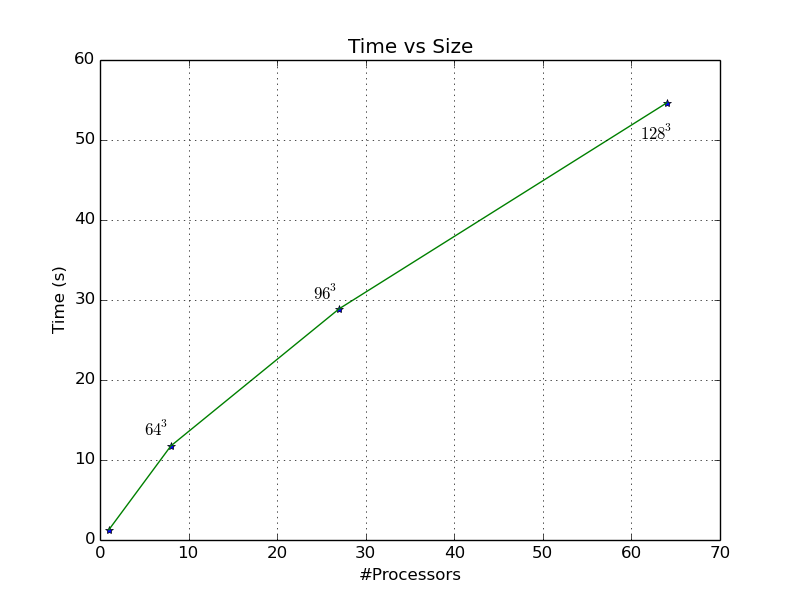
\includegraphics[width = 0.7\textwidth]{figures/scalingMG}
		\caption{A Langmuir Oscillation were performed for \(10\) timesteps with a \((32,32,32)\) grid on each processor.
		This was repeated with increasing amount of processors, \((1, 8, 32, 64)\), to see how the multigrid solver scales.}
		% \end{subfigure}
	\end{figure}
\end{frame}

\section{Concluding Remarks}
\begin{frame}
\frametitle{Concluding Remarks}
What was found.
	\begin{itemize}
		\item The multigrid solver was shown to work correctly
		\item The PINC was shown to work correctly
		\item Scalability was not shown to work satisfactorily
	\end{itemize}
\end{frame}

\begin{frame}
	\frametitle{Concluding Remarks}
	Next step
	\begin{itemize}
		\item More testing on PINC
		\item Solve the scaling issue shown
		\item Add more possibilities to PINC (already underway)
		\item Different Boundary Conditions are not well tested 
	\end{itemize}
\end{frame}

\section{Bibliography}
\begin{frame}
	\printbibliography
\end{frame}

\end{document}
